\documentclass[11pt]{article}

\usepackage[spanish,activeacute]{babel}
\usepackage{titlesec}
\usepackage{graphicx}
\usepackage{float}
\usepackage{subfig}
\usepackage{chngcntr}
\usepackage{xcolor}
\usepackage{listofitems}
\usepackage[bottom]{footmisc}
\usepackage[hidelinks]{hyperref}
\usepackage[most]{tcolorbox}


\setlength{\parindent}{1.0em}
\setlength{\parskip}{1.0em}
\setlength{\emergencystretch}{5.0em}
\setlength{\belowcaptionskip}{-10pt}
\counterwithin{figure}{section}
\titlespacing*{\section}{0em}{3.5em}{1.5em}
\setcounter{tocdepth}{1}
\hypersetup{
	linktoc=all
}


\title{\Huge Software en formato fuente}
\author{Eugenia Damonte, Ariel Fideleff y Mart\'in Go\~ni}
\date{}

\definecolor{fuchsia-vim}{RGB}{168,0,168}
\definecolor{orange-desert-vim}{RGB}{168,87,0}
\definecolor{darkgray}{RGB}{100,100,100}
\definecolor{light-blue}{RGB}{64, 76, 201}
\definecolor{light-red}{RGB}{201, 60, 60}
\definecolor{light-green}{RGB}{65, 181, 104}

\newtcolorbox{code-box}{colback=white!75!gray,colframe=white!15!gray,fontupper=\linespread{1.15}\selectfont}

\newcommand{\codetext}[2]{\large\texttt{\textcolor{#1}{#2}}}
\newcommand{\imagecaption}[1]{\vspace{-7pt}\caption*{\char91\ref{fig:#1}\char93}}


\begin{document}
	\pagenumbering{gobble}
	\maketitle
	\newpage
	\tableofcontents
	\newpage
	\pagenumbering{arabic}
	
	
	\section{Configuraci\'on previa}
		Antes de comenzar a resolver los ejercicios configuramos \texttt{vim} para editar archivos en C. Para hacer esto abrimos el archivo \texttt{\textasciitilde/.vimrc} (en todo caso de no existir, hay que crearlo) que es el archivo de configuraci'on de \texttt{vim}. Estaba vac'io por lo que le le a'nad'imos dos l'ineas: \texttt{set nocp} y \texttt{filetype plugin on}. Lo que hace el primer comando es desactivar el modo de compatibilidad. 'Este hace que algunas de las funciones de \texttt{vim} sean deshabilitadas o modificadas para que se comporte de manera similar a \texttt{vi}, el antecesor de \texttt{vim}. La segunda permite utlizar el plugin \texttt{filetype}.
		
		Luego para asegurarnos de tener todos los paquetes de \texttt{vim} utlizamos el comando \texttt{sudo apt-get install vim-gui-common vim-runtime}. El primer paquete tuvo que instalarse demorando varios minutos por la velocidad de descarga abismal de los repositorios. El segundo, por el otro lado ya estaba instalado en nuestro caso.
		
		Finalmente creamos el archivo de configuraci'on para los archivos con extensi'on \texttt{.c}, llamado \texttt{c.vim}. Para poder crearlo primero tuvimos que crear la carpeta \texttt{\textasciitilde/.vim/ftplugin}, que es donde se ponen los archivos de configuraci'on. Luego abrimos el mismo con \texttt{vim} y escribimos las configuraciones que quer'iamos usar.
		
		
		\begin{figure}[H]
			\centering
			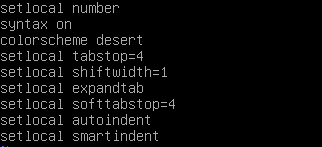
\includegraphics[width=.7\linewidth]{Images/Preamble/Preamble.PNG}
			\caption{Las configuraciones para los archivos \texttt{.c}}
			\label{fig:vim-setup}
		\end{figure}
		
		
	\section{Uso b'asico de gcc}
		Antes de comenzar con el proyecto en s'i, decidimos asegurarnos de que \texttt{gcc} funcionaba correctamente y que sab'iamos usarlo. Para hacer esto copiamos el programa de ejemplo, \texttt{circulo.c}, que se encuentra en el apunte provisto.
		
		\begin{figure}[H]
			\centering
			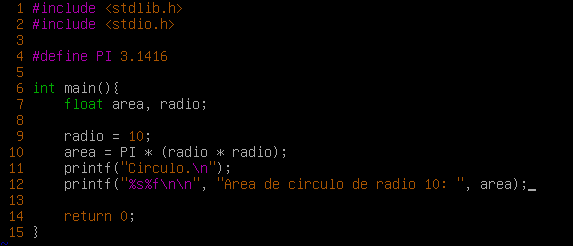
\includegraphics[width=.9\linewidth]{Images/Seccion 1/S1}
			\caption{El programa de ejemplo \texttt{circulo.c}}
		\end{figure}
		
	\subsection{Compilaci'on directa}
		Una vez copiado el programa realizamos una compilaci'on directa para asegurarnos de que el programa funcionase correctamente. Para hacer esto usamos el comando \texttt{gcc -o circulo circulo.c}. Lo que hace el argumento \texttt{-o} es permitirnos especificar el nombre delarchivo de salida, pues si no, el archivo se nombra por defecto \texttt{a.out}.
		
		\begin{figure}[H]
			\centering
			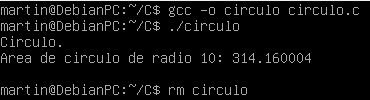
\includegraphics[width=.7\linewidth]{Images/Seccion 1/S1 parte dos}
			\caption{Muestra del funcionamiento de \texttt{circulo.c}}
			\label{fig:basic-compilation}
		\end{figure}
		
	\subsection{Compilaci'on compleja}
		Habiendo comprobado que \texttt{gcc} funcionaba correctamente decidimos intentar compilar el mismo archivo, \texttt{circulo.c}, de manera compleja. Es decir, haciendo cada uno de los pasos que realiza el compilador a la hora de transformar un archivo en C en un programa ejecutable, manualmente uno por uno.
	
	\subsubsection{Preprocesamiento}
		El preprocesado o preprocesamiento es la primera etapa de modificaci'on del c'odigo fuente. Sirve para que, en la fase de compilaci'on, que es la siguiente, el compilador pueda leer correctamente el c'odigo. 
    
    	El trabajo del preprocesador consiste en llevar a cabo las instrucciones dadas por las \textit{directivas} dirigidas al mismo (que, en el caso de C y C++, son las que comienzan con un numeral, como \texttt{\textcolor{fuchsia-vim}{\#define}}, \texttt{\textcolor{fuchsia-vim}{\#include}}, \texttt{\textcolor{fuchsia-vim}{\#ifdef}} y \texttt{\textcolor{fuchsia-vim}{\#error}}, entre otros).

   		En el archivo \texttt{circulo.c} podemos encontrar la directiva  \texttt{\textcolor{fuchsia-vim}{\#define PI} \textcolor{orange-desert-vim}{3.1416}}, que justamente define una constante de nombre \texttt{\textcolor{fuchsia-vim}{PI}} y valor \texttt{\textcolor{orange-desert-vim}{3.1416}}. Esta constante es llamada en la funci'on \texttt{main} de manera que, en vez de escribir  \texttt{\textcolor{orange-desert-vim}{3.1416}}, escribimos simplemente  \texttt{\textcolor{fuchsia-vim}{PI}}.

    	En la figura \ref{fig:preproc_circ},
   		se observa el c'odigo preprocesado que obtuvimos como salida del comando \texttt{gcc -E circulo.c} (tambi'en se puede usar \texttt{cpp circulo.c}, que hace referencia directamente al preprocesador). Si prestamos atenci'on, la directiva antes mencionada no figura en esta salida. Adem'as, en la l'inea que en el c'odigo fuente dec'ia \texttt{\textcolor{darkgray}{area = PI * (radio * radio)}}, ahora dice \texttt{\textcolor{darkgray}{area = \textcolor{orange-desert-vim}{3.1416} * (radio * radio)}}. 

   		En resumen, lo que hizo el preprocesador fue tomar esa definici'on que le indicamos en la directiva y coloc'o el valor de la constante en las partes del c'odigo en donde se hac'ia referencia a ella.
   		
   		\begin{figure}[H]
   			\centering
			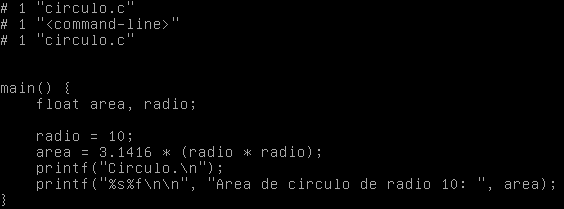
\includegraphics[width=.9\linewidth]{Images/Seccion 1/preprocesado_circulo}
   			\caption{Resultado del preprocesado de \texttt{circulo.c}}
   			\label{fig:preproc_circ}
   		\end{figure}

	\subsubsection{Compilaci'on}
		La compilaci'on es el proceso donde se transforma el c'odigo antes preprocesado (en nuestro caso en C), a assembler propio del procesador de la computadora (en espa'nol, \textit{lenguaje ensamblador}). Para hacer esto usamos el comando \texttt{gcc -S circulo.c}. Notar que directamente nos referimos al archivo con el c'odigo fuente \texttt{circulo.c}, pues el argumento \texttt{-S} ya de por medio realiza el preprocesado antes explicado. Finalmente verificamos que haya funcionado el comando, mostrando las primeras l'ineas del archivo \texttt{circulo.s}, que es donde \texttt{gcc} almacena el compilado.

		\begin{figure}[H]
			\centering
			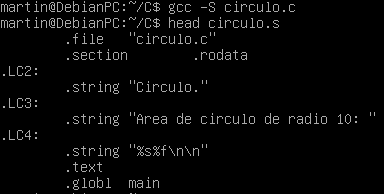
\includegraphics[width=.7\linewidth]{Images/Seccion 1/S1 parte tres.PNG}
			\caption{Primeras 10 l'ineas del resultado de la compilaci'on}
			\label{fig:complex-compilation}
		\end{figure}
		
	\subsubsection{Ensamblado}
		Una vez realizado el compilado, procedemos a ensamblar el archivo. Es decir, transformar el archivo de assembler a c'odigo objeto, un archivo binario en lenguaje m'aquina. Hicimos esto con el comando \texttt{as -o circulo.o circulo.s}. Luego verificamos que haya funcionado revisando qu'e tipo de archivo era \texttt{circulo.o} haciendo uso del comando \texttt{file}.
		
		Aclarar que otra forma por la cual podr'iamos haber obtenido el archivo en cuesti'on ser'ia el comando \texttt{gcc -c circulo.c}, pero como se puede ver, toma directamente desde el c'odigo fuente, ya que adem'as realiza todas las etapas previas explicadas.
		
		\begin{figure}[H]
			\centering
			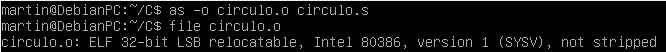
\includegraphics[width=.9\linewidth]{Images/Seccion 1/S1 parte cuatro}
			\caption{Ejecuci'on del ensamblado y detalles del archivo generado}
			\label{fig:complex-assembly}
		\end{figure}
	
		Al estar el archivo conseguido en lenguaje m'aquina, no es texto en s'i que podamos ver con facilidad. En todo caso, podemos hacer uso de un comando como lo es \texttt{objdump -d circulo.o}, que intepreta y permite ver las instrucciones a la computadora contenidas en el archivo. Hay que aclarar que las posiciones de memoria a las que se refiere probablemente no sean correctas, ya que 'estas deben ser relacionadas en el pr'oximo paso, el enlazado, con las librer'ias externas utilizadas.
		
	\subsubsection{Enlazado}
		Finalmente enlazamos el archivo. El enlazado es el proceso mediante el cual se vincula y se incorpora al programa, las librerias que requiere para poder funcionar. Estas librerias est'an compuestas de c'odigo con funciones que uno utiliza en dicho programa. Por ejemplo, en \texttt{circulo.c} usamos funciones como \texttt{\textcolor{darkgray}{printf}}, el cual hace referencia a la libreria \texttt{stdio.h} (t'ipicamente se definir'ia al comienzo del programa de la forma \texttt{\textcolor{fuchsia-vim}{\#include}\textcolor{orange-desert-vim}{\char60stdio.h\char62}} pero, al ser com'unmente utilizado, es incorporado autom'aticamente por el compilador).
		
		En este paso es donde nos encontramos con problemas. El comando que se da en el apunte no funciona. Al usarlo da varios errores indicando que las librerias usadas como argumentos no existen, as'i como tambi'en con algunas de las opciones del comando.
	
		\begin{figure}[H]
			\centering
			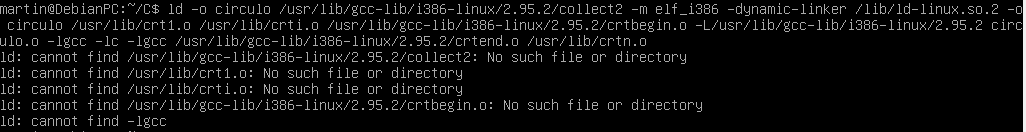
\includegraphics[width=.9\linewidth]{Images/Seccion 1/S1 parte cinco}
			\caption{El primer intento de usar \texttt{ld}, siguiendo el apunte}
			\label{fig:first-ld-attempt}
		\end{figure}
		
		Dado todos los errores que hab'ian, decidimos borrar todas las opciones innecesarias y probar nuevamente. Al hacer esto, los errores anteriores desaparecieron a cambio de uno nuevo. 'Este dec'ia ``\texttt{cannot find entry symbol \textunderscore\/start}'', el cual se traduce como ``\texttt{no se encuentra el simbolo de entrada \textunderscore\/start}''. Luego de algo de investigar descubrimos que este error se debe a que el verdadero punto de entrada\footnotemark\/ de un programa es \texttt{\textunderscore\/start} y no \texttt{main}, siendo que \texttt{\textunderscore\/start} simplemente redirige a 'el. Para solucionar esto usamos el argumento \texttt{--entry main} para especificar la funci'on \texttt{main} como el punto de entrada del programa.
		
		\footnotetext{El punto de entrada de un programa es donde se ejecutan las primeras instrucciones y se pasa control al programa.}
		
		Una vez hechos estos cambios la funci'on no daba mas errores y el programa parec'ia estar listo para usar. A la hora de ejecutarlo, sin embargo, 'este no era reconocido como un programa ejecutable. Para asegurarnos de haber hecho todo correctamente revisamos que el archivo existiese as'i como tambi'en sus permisos, siendo 'estos correctos.
		
		\begin{figure}[H]
			\centering
			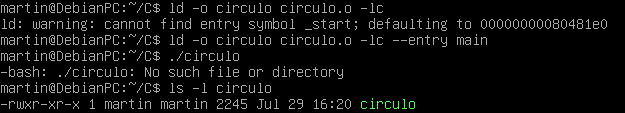
\includegraphics[width=.9\linewidth]{Images/Seccion 1/S1 parte seis}
			\caption{El segundo intento de usar \texttt{ld}}
			\label{fig:second-ld-attempt}
		\end{figure}
		
		Dado que no pod'iamos ejecutar el programa decidimos intentar volver a a'nadir algunas de las opciones que no causaban ores. Primero volvimos a a'nadir las opciones \texttt{-m elf\textunderscore\/i386} y \texttt{--dynamic-linker /lib/ld-linux.so.2}. La primera opci'on define el objetivo del compilador\footnotemark. La segunda define la ubicaci'on del enlazador din'amico\footnotemark\/ a usar.
		
		\footnotetext{El objetivo del compilador es lo que determina que tipo de c'odigo objeto debe producir la funci'on.}
		\footnotetext{Un enlazador din'amico o \textit{dynamic linker} es una forma de enlazar los archivos binarios que se necesitan para que el programa funcione. En este caso el c'odigo de las funciones se mantienen en la biblioteca y la hora de ejecutar el programa se cargan en memoria.}
		
		Luego de hacer estos cambios logramos ejecutar el programa, que parec'ia funcionar correctamente. Sin embargo, al final de 'este tuvimos el error \texttt{Segmentation fault}. Para tratar de averiguar de donde ven'ia el error decidimos debuggear el programa utilizando \texttt{gdb}.
		
		\begin{figure}[H]
			\centering
			\subfloat[Error al correr el programa]{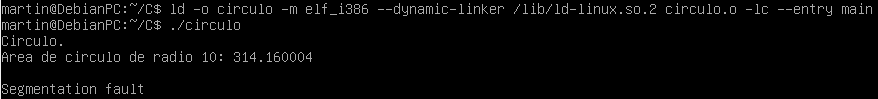
\includegraphics[width=.8\linewidth]{Images/Seccion 1/S1 parte siete}} \par
			\subfloat[Nuestro intento de debuggear el programa]{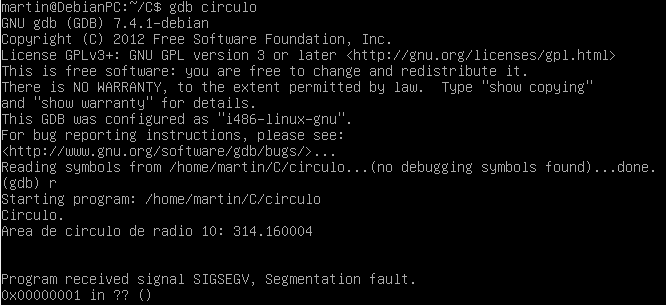
\includegraphics[width=.8\linewidth]{Images/Seccion 1/S1 parte ocho}}
			
			\caption{El tercer intento de usar \texttt{ld}}
			\label{fig:third-ld-attempt}
		\end{figure}
		
		Cuando intentamos debuggear el programa nos encontramos con algo extra'no, y es que \texttt{gdb} no sab'ia de qu'e l'inea proven'ia el error. Esto nos llev'o a creer que proven'ia del enlazado del programa, y no del programa en s'i. Luego de buscar m'as todav'ia, encontramos el problema, y es que nos faltaba incluir las librerias que requer'ia el enlazador din'amico. Para entender por qu'e pasa esto hay que entender c'omo funciona el comando.
		
		Lo primero que hace el comando es especificar la ubicaci'on del enlazador din'amico que requieren las dem'as librerias para acceder a las funciones din'amicas de C. Luego se incluyen otras tres librerias \texttt{/usr/lib/i386-linux-gnu/crt1.o}, \texttt{/usr/lib/i386-linux-gnu/crti.o} y \texttt{/usr/lib/i386-linux-gnu/crtn.o}. La primera es la librer'ia que tiene referencias a los archivos que requiere el enlazador (\texttt{/lib/libc.so.6} y \texttt{/usr/lib/libc\textunderscore\/nonshared.a}). Las otras dos se encargan de que existan \texttt{\textunderscore\/init} y \texttt{\textunderscore\/fini}, que son el c'odigo de inicializaci'on y finalizaci'on. Algo importante de recordar es que la ubicaci'on de las librerias puede cambiar dependiendo del sistema y la instalaci'on especifica. En nuestro caso, las encontramos buscando en \texttt{/usr/lib} y revisando todas las carpetas que parec'ian tener alguna relaci'on.
	
		Es importante notar la posici'on de las librer'ias, \texttt{crti.o} debe ir despu'es de \texttt{crt1.o}. Esto es porque el segundo hace referencia al primero. Adem'as ambas deben ir antes del archivo que se est'a enlazando. Finalmente \texttt{crtn.o} va al final del comando, despu'es de todos los dem'as argumentos.
		
		\begin{figure}[H]
			\centering
			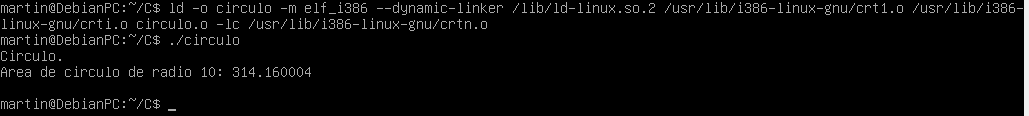
\includegraphics[width=.9\linewidth]{Images/Seccion 1/S1 parte nueve.PNG}
			\caption{El cuarto y 'ultimo intento de usar \texttt{ld}}
			\label{fig:fourth-ld-attempt}
		\end{figure}
		
		Luego de hacer todo esto, el programa finalmente funcion'o y se ejecut'o de manera correcta y sin errores. Habiendo terminado decidimos que ya ten'iamos el suficiente conocimiento para intentar compilar un programa usando \texttt{make}.
		
		
	\section{Uso b'asico de make}
	\subsection{Bases de make}
		El programa \texttt{make} es una herramienta que permite manejar y mantener programas que constan de muchos archivos y tienen m'ultiples dependencias. Este evita tener que volver a recompilar el programa manualmente cada ves que se hacen cambios. Autom'aticamente detecta qu'e archivos necesitan ser recompilados y da las instrucciones para hacerlo, todo con un solo comando.
		
		La base del sistema esta un archivo llamado \texttt{makefile}, en este se almacenan las instrucciones que \texttt{make} utiliza a la hora de compilar un programa. Este contiene las reglas de dependencia, macros y las reglas impl'icitas. Las reglas de dependencia son reglas que definen que archivos son necesarios para crear un objetivo\footnotemark. Los macros son variables que almacenan un valor determinado, son muy `utiles para evitar repetir arguementos una gran cantidad de veces. Finalmente las reglas impl'icitas, estas son una manera de especificar reglas o condiciones usadas a la hora de compilar el programa.
		
		\footnotetext{Un objetivo es el nombre de un archivo(ejecutable o  objeto) o una acci'on de ese \texttt{makefile}.} 

	\subsection{Compilaci'on simple con make}
		Para asegurarnos de que sab'iamos usar make decidimos compilar el programa de ejemplo que aparece en el apunte, la calculadora con notaci'on polaca. Primero tuvimos que llevar los archivos a la m'aquina virtual, para hacer esto los descargamos de la p'agina web mencionada en el apunte utilizando \texttt{wget}.
		
		\begin{figure}[H]
				\centering
				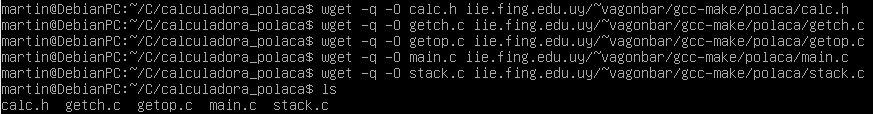
\includegraphics[width=.9\linewidth]{Images/Seccion 2/S2.PNG}
				\caption{Descargamos los archivos a la MV}
				\label{fig:makefile-download}
		\end{figure}
		
		Una vez descargados todos los archivos compilamos el programa sin utlizar \texttt{make} para asegurarnos de que este funcionase correctamente. Para hacer esto usamos \texttt{gcc}, dandole como argumento todos los archivos que necesitaban ser compilados.
		
		\begin{figure}[H]
				\centering
				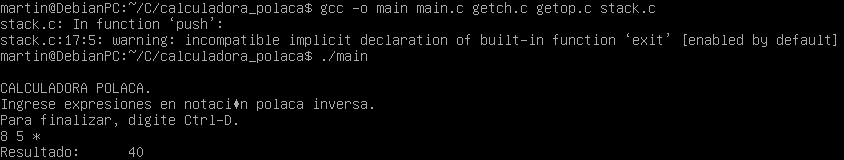
\includegraphics[width=.9\linewidth]{Images/Seccion 2/S2 parte dos.PNG}
				\caption{Compilamos el programa sin \texttt{make}}
				\label{fig:makefile-gcc-compile}
		\end{figure}
	
		Habiendo confirmado que el programa funcionaba creamos el archivo \texttt{makefile}, necesario para que make funcione. En este colocamos todas las reglas necesarias para compilar el programa. Estas especificaban que se deb'ia hacer con cada archivo. Para hacer esto usamos reglas de dependencia, estas siguen la siguiente estructura:
		
		%Agrande un poco la letra por cuestiones esteticas. Cambienlo si no les parece.
		\begin{figure}[H]
			\centering
			\begin{code-box}
				\codetext{light-blue}{\Large destino} : \codetext{orange-desert-vim}{ \Large dependencias}
				
				\qquad\codetext{light-red}{\Large comando}
			\end{code-box}
		\end{figure}
		
		Donde \texttt{\textcolor{light-blue}{destino}} es el nombre del archivo a donde ira el resultado de las acciones de \texttt{\textcolor{light-red}{comando}}. Es importante notar que \texttt{\textcolor{light-blue}{destino}} tambi'en puede ser una acci'on que puede ser llamada desde el archivo o al usar \texttt{make}. Luego tenemos dependencias, son los archivos que se usan para crear \texttt{\textcolor{orange-desert-vim}{destino}} y deben estar presentes en la ubicaci'on especificada. Finalmente esta \texttt{\textcolor{light-red}{comando}}, son comandos enviados a el shell para ser interpretados. Pueden tambi'en ser acciones del archivo.
		
		\begin{figure}[H]
			\centering
			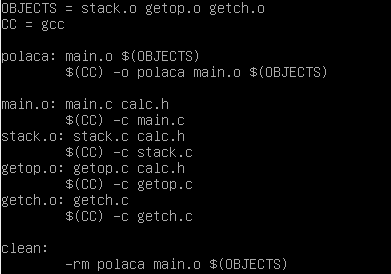
\includegraphics[width=.9\linewidth]{Images/Seccion 2/S2 parte tres.PNG}
			\caption{El \texttt{makefile} creado para compilar el programa}
			\label{fig:makefile}
		\end{figure}
		
		Sabiendo como crear reglas de dependencia y con ayuda del apunte creamos el \texttt{makefile} necesario para compilar el programa. Tiene adem'as una acci'on para eliminar el archivo ejecutado y todos los archivos \texttt{.o} generados por la compilaci'on.
		
		Al ejecutar el comando \texttt{make polaca} para compilar el programa, este se ejecut'o exitosamente y sin errores. Para verificar que todo funcionase correctamente realizamos la misma operación que habíamos realizado al compilar el programa la primera vez. Al ver que los resultados eran iguales y el programa funcionaba correctamente dimos por terminada la practica con \texttt{make}. Antes de pasar a compilar \texttt{w3m} borramos todos los archivos innecesarios con \texttt{make clean}.
		
		\begin{figure}[H]
			\centering
			\subfloat[Compilamos y ejecutamos el programa]{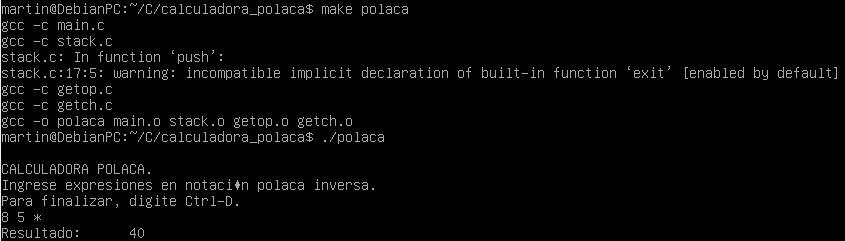
\includegraphics[width=.8\linewidth]{Images/Seccion 2/S2 parte cuatro}} \par
			\subfloat[Borramos todos los archivos innecesarios]{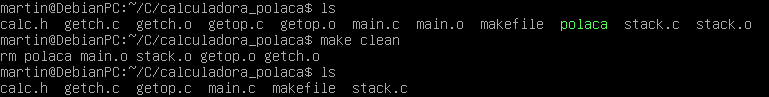
\includegraphics[width=.8\linewidth]{Images/Seccion 2/S2 parte cinco}}
			
			\caption{El comando \texttt{make} en funcionamiento}
			\label{fig:makefile-successful-compile}
		\end{figure}
		
		
	\section{Compilando con make}
	
	Para poder llevar m'as a la pr'actica el conocimiento del funcionamiento de \texttt{make} y la compilaci'on de programas mediante makefiles, compilaremos \texttt{w3m}, un navegador web que funciona dentro de la terminal.
	
	Descargamos el c'odigo fuente\footnote{\url{https://sourceforge.net/projects/w3m/files/}}, los archivos necesarios para el proceso, y notamos que se encuentran en un archivo del tipo \texttt{.tar.gz}\footnote{Un archivo \texttt{.tar} es utilizado para almacenar m'ultiples archivos y directorios en un solo archivo. Y luego el sufijo \texttt{.gz} muestra que los contenidos de dicho se encuentran comprimidos, y la forma en que fueron comprimidos.}. Para extraer sus contenidos, podemos usar el comando \texttt{tar} de linux, aunque para ello primero debemos instalarlo usando \texttt{sudo apt-get install tar}. Hecho esto, el comando utilizado para extraer los archivos es \texttt{tar -xf w3m-0.5.3.tar.gz}, donde \texttt{-x} implica extraer los archivos, y \texttt{-f} dice que se ejecuten las acciones sobre un archivo cuya ruta se encuentra a continuaci'on de la opci'on. Por el nombre del archivo, es claro que la versi'on de \texttt{w3m} descargada es la \texttt{0.5.3}. Al descomprimir nos queda en el lugar de extracci'on, una carpeta llamada \texttt{w3m-0.5.3} con todos los archivos.
	
	Al abrir la carpeta, vemos la presencia de distintos archivos, entre ellos podemos notar algunos \texttt{.c} o \texttt{.h}, que como sabemos corresponden a c'odigo hecho en el lenguaje C. Para saber c'omo proceder, nos dirigimos como es habitual al archivo \texttt{README} presente. En 'el nos dice que nos dirijamos a la subcarpeta \texttt{doc} para las instrucciones en ingl'es. Vemos que all'i se encuentra otro \texttt{README} con una breve descripci'on del programa y las instrucciones dichas. Indica que primero ejecutemos el archivo \texttt{configure}, presente en la carpeta ra'iz, de la forma \texttt{./configure}. Aqu'i empiezan los problemas.
	
	\begin{figure}[H]
		\centering
		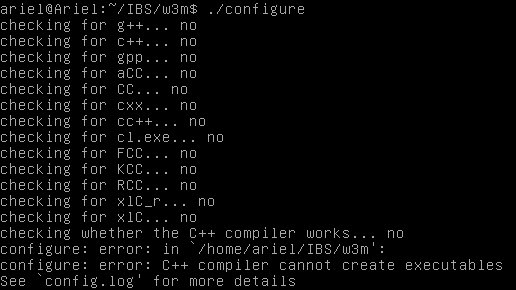
\includegraphics[width=.8\linewidth]{Images/Compile_w3m/g++_missing}
		\caption{Primer intento de ejecuci'on de \texttt{configure}}
	\end{figure}
	
	Al ejecutar configure, nos dice \texttt{C++ compiler cannot create executables}, es decir, como que el compilador de C++ no puede crear ejecutables, y tambi'en que para m'as detalles podemos revisar el archivo generado \texttt{config.log}. All'i se puede ver todo el historial de las acciones realizadas por \texttt{configure}, y notamos que verifica por la presencia de ciertos programas, que parecen ser todos compiladores de C++, pudiendo significar que no existe ninguno en la m'aquina.
	
	\begin{figure}[H]
		\centering \captionsetup{justification=centering}
		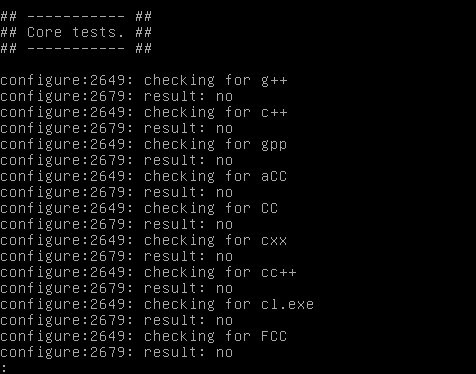
\includegraphics[width=.7\linewidth]{Images/Compile_w3m/g++_missing_log}
		\caption{Contenidos de \texttt{configure.log} luego del primer intento de ejecuci'on de \texttt{configure}}
	\end{figure}
	
	Instalamos entones el primero de entre los que prueba, \texttt{g++}, de la forma \texttt{sudo apt-get install g++}. Esta vez, al correr \texttt{configure} parece lograr mayor progreso que la anterior, pero de todas formas a'un la ejecuci'on presenta otro error: \texttt{configure: error: gc.h not found}.
	
	\begin{figure}[H]
		\centering \captionsetup{justification=centering}
		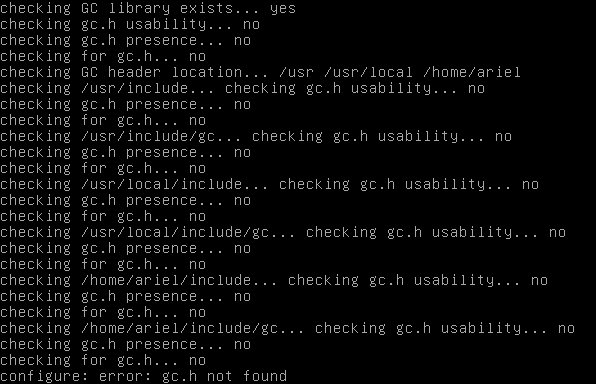
\includegraphics[width=.8\linewidth]{Images/Compile_w3m/gc_missing}
		\caption{Segundo intento de ejecuci'on de \texttt{configure}}
	\end{figure}
	
	Estuvimos investigando este problema, viendo c'omo se puede obtener este archivo que parece faltar. Notamos que verifica por la existencia del archivo mencionado en m'ultiples rutas antes de mostrar el error. Luego de buscar un poco, parece ser lo que se llama el ``Garbage Collector'', que es lo que usan m'ultiples lenguajes de programaci'on como mecanismo para la gesti'on adecuada de la memoria, y as'i tanto reservar espacios de dicha memoria, liberarlos, tener cuenta del espacio libre y ocupado, e incluso la reorganizaci'on del mismo a fin de liberar el mayor espacio posible que pueda ser utilizado, compactando los espacios de memoria libres entre los ocupados, dejando la mayor cantidad contigua libre posible. 
	
	Despu'es de saltar mucho entre p'aginas investigando, llegamos a una con informaci'on detallada sobre las dependencias que uno puede instalar en Linux, en espec'ifico la de \texttt{libgc-dev}\footnote{\url{https://ubuntu.pkgs.org/16.04/ubuntu-main-amd64/libgc-dev_7.4.2-7.3_amd64.deb.html}} ya que vimos que contiene entre sus archivos, el archivo \texttt{gc.h} faltante. Entonces irectamente lo instalamos de la forma \texttt{sudo apt-get install libgc-dev}.
	
	Probamos nuevamente correr \texttt{configure}, y por lo que vimos, pareci'o finalizar sin inconvenientes.
	
	\begin{figure}[H]
		\centering \captionsetup{justification=centering}
		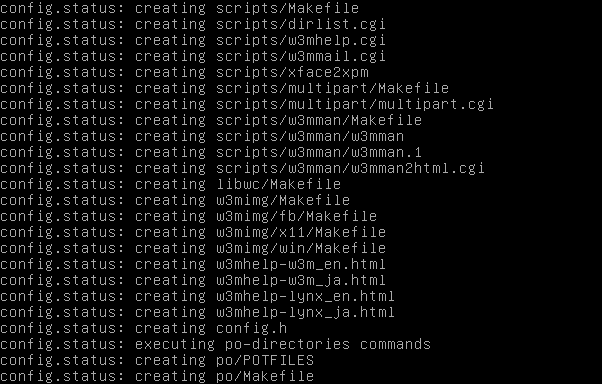
\includegraphics[width=.8\linewidth]{Images/Compile_w3m/configure_successful}
		\caption{Tercer intento (y correcto) de ejecuci'on de \texttt{configure}}
	\end{figure}
	
	Dado esto, pudimos proceder al siguiente paso: correr el makefile para compilar, usando el comando \texttt{make} en el directorio ra'iz. Y como era de esperarse, hubo problemas tambi'en en este paso.
	
	\begin{figure}[H]
		\centering \captionsetup{justification=centering}
		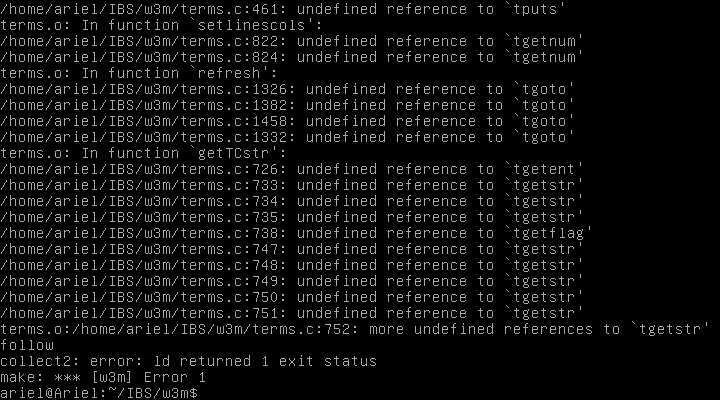
\includegraphics[width=.8\linewidth]{Images/Compile_w3m/libtinfo-dev_missing}
		\caption{Primer intento de ejecuci'on del makefile}
	\end{figure}
	
	Viendo que el compilador no pudo encontrar las referencias de una serie de funciones utilizadas como \texttt{\textcolor{darkgray}{tputstring}} y otros con nombres similares, luego de buscar un poco, 'estas podr'ian estar presentes en el paquete \texttt{libtinfo-dev}, el cual instalamos de la forma \texttt{sudo apt-get install libtinfo-dev}. Probamos nuevamente entonces correr \texttt{make}.
	
	De todas formas, dada la rapidez con la que corri'o en comparaci'on a la anterior ejecuci'on, sumado a que se presentan los mismos errores que dicha vez, probamos en cambio primero probar con correr \texttt{configure} otra vez, y luego \texttt{make}.
	
	%No había hecho captura cuando pensé que si :(
	
	Comprobamos que el error antes experimentado desapareci'o, a cambio de otro nuevo:\enspace\verb|cannot stat `t-ja.gmo': No such file or directory| Nuevamente investigamos este error y encontramos en un foro que un error id'entico se le presenta a un usuario cuando quiso instalar otro paquete\footnote{ \url{https://www.linuxquestions.org/questions/linux-general-1/alsa-utils-failing-make-stage-cannot-stat-\%60t-ja-gmo\%27-i-think-i-need-xgettext-386546/}}, y que se puede resolver instalando el paquete \texttt{gettext}, de la forma \texttt{sudo apt-get install gettext}. Una vez instalado, al igual que antes volvemos a correr \texttt{configure} y \texttt{make}.
	
	\begin{figure}[H]
		\centering \captionsetup{justification=centering}
		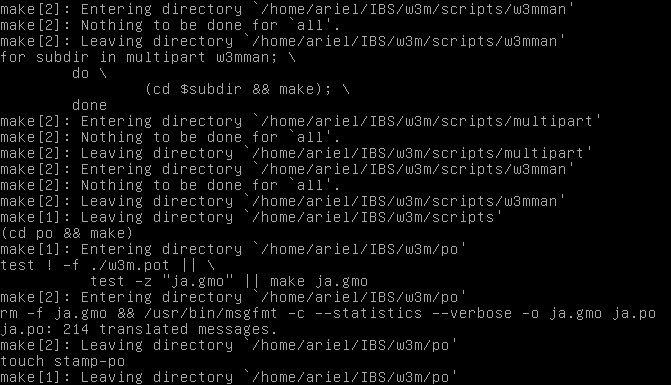
\includegraphics[width=.8\linewidth]{Images/Compile_w3m/make_successful}
		\caption{Segundo intento (y correcto) de ejecuci'on del makefile}
	\end{figure}
	
	Esta vez parece no haber ning'un error visible. Entonces procedemos al paso final, a lo que corremos \texttt{make install}.
	
	\begin{figure}[H]
		\centering \captionsetup{justification=centering}
		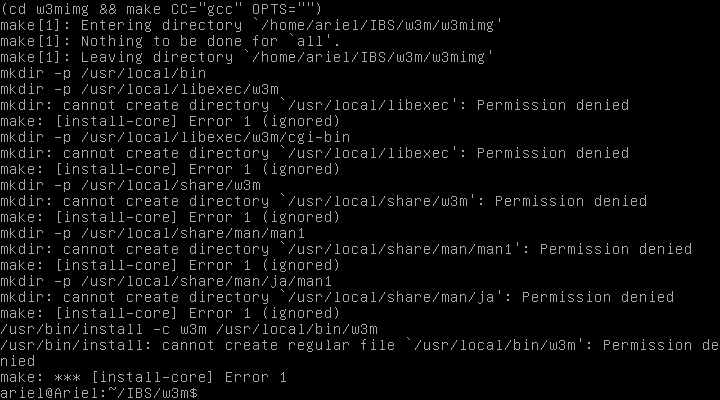
\includegraphics[width=.8\linewidth]{Images/Compile_w3m/make-install_fail}
		\caption{Primer intento fallido de ejecuci'on de \texttt{make install}}
	\end{figure}
	
	Experimentamos una serie de \texttt{Permission denied}, por lo que lo m'as probable es que para correr este comando, requerimos permisos root. Por lo tanto, probamos agregar \texttt{sudo}, al comienzo del comando.
	
	\begin{figure}[H]
		\centering \captionsetup{justification=centering}
		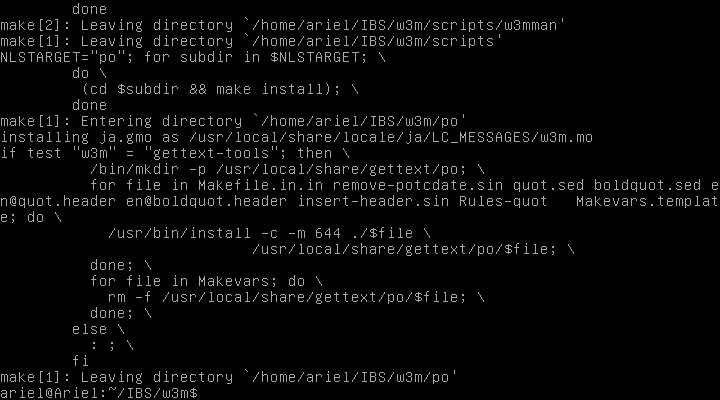
\includegraphics[width=.8\linewidth]{Images/Compile_w3m/make-install_successful}
		\caption{Segundo intento (y correcto) de ejecuci'on de \texttt{make install}}
	\end{figure}
	
	Ning'un error visible. 'Este habr'ia sido el 'ultimo paso de la instalaci'on, y deber'iamos ser capaces de correr \texttt{w3m} correctamente. Para probar su funcionamiento, probamos entrar a \url{www.google.com} con el comando \texttt{w3m www.google.com}.
	
	\begin{figure}[H]
		\centering \captionsetup{justification=centering}
		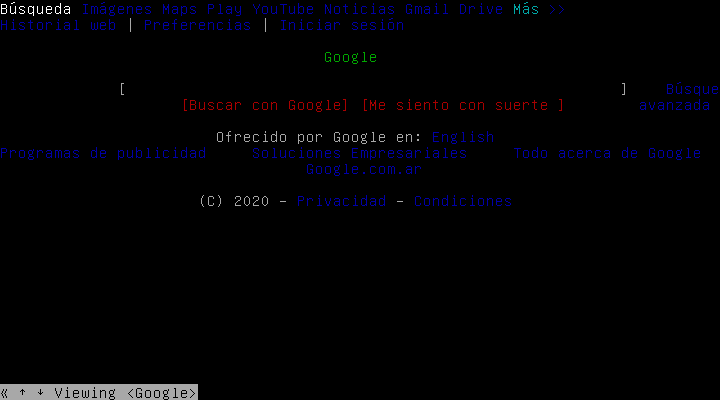
\includegraphics[width=.8\linewidth]{Images/Compile_w3m/test_w3m}
		\caption{Entrando a \url{www.google.com} con \texttt{w3m}}
	\end{figure}
	
	¡Y efectivamente podemos visualizar el sitio web sin problemas! Pudimos compilar correctamente \texttt{w3m}.
		
	\section{Comandos usados}
		A continuaci'on se encuentran todos los comandos utilizados en este trabajo, correspondientes a las im'agenes presentadas.
		
		\begin{figure}[H]
			\centering
			\begin{code-box}
				\codetext{light-blue}{setlocal} \codetext{light-red}{number}
				
				\codetext{light-blue}{syntax} \codetext{light-red}{on}

				\codetext{light-blue}{colorscheme} \codetext{light-red}{desert}
				
				\codetext{light-blue}{setlocal} \codetext{light-red}{tabstop=4}

				\codetext{light-blue}{setlocal} \codetext{light-red}{shiftwidth=1}
				
				\codetext{light-blue}{setlocal} \codetext{light-red}{expandtab}
				
				\codetext{light-blue}{setlocal} \codetext{light-red}{softtabstop=4}
				
				\codetext{light-blue}{setlocal} \codetext{light-red}{autdoindent}
				
				\codetext{light-blue}{setlocal} \codetext{light-red}{smartindent}
			\end{code-box}
			\imagecaption{vim-setup}
		\end{figure}
		
		\begin{figure}[H]
			\centering
			\begin{code-box}
				\codetext{light-blue}{gcc} \codetext{orange-desert-vim}{-S} \codetext{light-red}{circulo.c}
				
				\codetext{light-blue}{head} \codetext{light-red}{circulo.s}
			\end{code-box}
			\imagecaption{complex-compilation}
		\end{figure}
		
		\begin{figure}[H]
			\centering
			\begin{code-box}
				\codetext{light-blue}{as} \codetext{orange-desert-vim}{-o circulo.o} \codetext{light-red}{circulo.s}
				
				\codetext{light-blue}{file} \codetext{light-red}{circulo.o}
			\end{code-box}
			\imagecaption{complex-assembly}
		\end{figure}
		
		\begin{figure}[H]
			\centering
			\begin{code-box}
			\codetext{light-blue}{ld} \codetext{orange-desert-vim}{-o circulo /usr/lib/gcc-lib/i386-linux/2.95.2/ collect2 -m elf\textunderscore{}i386 --dynamic-linker /lib/ld-linux.so.2 -o circulo /usr/lib/crt1.o /usr/lib/crti.o /usr/lib/gcc-lib/i386-linux/2.95.2/ crtbegin.o -L /usr/lib/gcc-lib/i386-linux/2.95.2} \codetext{light-red}{circulo.o }\codetext{orange-desert-vim}{-lgcc -lc -lgcc /usr/lib/gcc-lib/ i386-linux/2.95.2/crtend.o /usr/lib/crtn.o}
			\end{code-box}
			\imagecaption{first-ld-attempt}
		\end{figure}
		
		\begin{figure}[H]
			\centering
			\begin{code-box}
				\codetext{light-blue}{ld} \codetext{orange-desert-vim}{-o circulo} \codetext{light-red}{circulo.o} \codetext{orange-desert-vim}{-lc}
				
				\codetext{light-blue}{ld} \codetext{orange-desert-vim}{-o circulo} \codetext{light-red}{circulo.o} \codetext{orange-desert-vim}{-lc --entry main}
				
				\codetext{light-blue}{./circulo}
				
				\codetext{light-blue}{ld} \codetext{orange-desert-vim}{-l} \codetext{light-red}{circulo}
			\end{code-box}
			\imagecaption{second-ld-attempt}
		\end{figure}
		
		\begin{figure}[H]
			\centering
			\begin{code-box}
				\codetext{light-blue}{ld} \codetext{orange-desert-vim}{-o circulo -m elf\textunderscore\/i386 --dynamic-linker /lib/ld-linux.so.2} \codetext{light-red}{circulo.o} \codetext{orange-desert-vim}{-lc --entry main}
				
				\codetext{light-blue}{./circulo}
				
				\codetext{light-blue}{gdb} \codetext{light-red}{circulo}
				
				\codetext{light-green}{(gdb)} \codetext{light-blue}{r}
			\end{code-box}
			\imagecaption{third-ld-attempt}
		\end{figure}
		
		\begin{figure}[H]
			\centering
			\begin{code-box}
				\codetext{light-blue}{ld }\codetext{orange-desert-vim}{-o circulo -m elf\textunderscore\/i386 --dynamic-linker /lib/ld-linux.so.2 /usr/lib/i386-linux-gnu/ crt1.o /usr/lib/i386-linux-gnu/crti.o} \codetext{light-red}{circulo.o} \codetext{orange-desert-vim}{-lc /usr/lib/i386-linux-gnu/crtn.o}
				
				\codetext{light-blue}{./circulo}
			\end{code-box}
			\imagecaption{fourth-ld-attempt}
		\end{figure}
		
		
		
		
		
		
		
		
		
		
				

		


















%Remove whitspace when done, for ease of work.
\end{document}
